\documentclass[10pt,journal,compsoc,onecolumn]{IEEEtran}
\usepackage[utf8]{inputenc}
\usepackage{amsmath,amsfonts,amssymb}
\usepackage{amsthm}
\usepackage{graphicx}
\usepackage{cite}
\usepackage{textcomp}
\usepackage{tikz}
\usetikzlibrary{arrows,positioning,shapes.geometric}
\usepackage{booktabs}
\usepackage{url}

\newtheorem{theorem}{Theorem}
\newtheorem{lemma}[theorem]{Lemma}
\newtheorem{definition}[theorem]{Definition}
\newtheorem{corollary}[theorem]{Corollary}

\begin{document}

\title{Algorithmic Foundations of Binary Trees: Hierarchical Topologies, Structural Taxonomies, Recursive Depth-First Traversals, and Breadth-First Level-Order View Projections}

\IEEEtitleabstractindextext{%
\begin{abstract}
This research paper provides an exhaustive formal investigation into the algorithmic foundations, mathematical properties, and traversal mechanics of Binary Tree data structures based on fundamental computational hierarchies. Contrasting non-linear hierarchical topologies with linear arrays and linked lists, we formalize primary metric invariants including node depth, subtree height, and level assignments. We establish a rigorous taxonomy across canonical tree archetypes—Full (Proper), Complete, and Perfect binary trees—deriving exact bounding theorems on level populations and cumulative node counts ($N = 2^{h+1} - 1$) via finite geometric progressions, while elucidating the zero-overhead contiguous array indexing ($2i+1, 2i+2$) enabled by complete trees. We systematically formalize the three classic recursive Depth-First Search (DFS) traversals—Pre-order, In-order, and Post-order—grounded in structural induction, establishing their $\Theta(N)$ runtime bounds and call-stack memory dynamics ($\Theta(H)$). Transitioning from deep recursion to iterative state machines, we formulate the Breadth-First Search (BFS) level-order traversal using First-In, First-Out (FIFO) queue abstractions, establishing its $\Theta(W)$ auxiliary width bound. Furthermore, we resolve the Left View and Right View boundary projection problems through both level-order partition filtering and depth-tracked DFS traversals. Granular execution trace tables, high-resolution vector TikZ architectural diagrams, multi-language reference implementations across Java, C++, and Python, and mappings to real-world industrial systems (compiler ASTs, B-Trees, and DOM virtual reconciliation) accompany all discussions.
\end{abstract}

\begin{IEEEkeywords}
Binary Trees, Hierarchical Data Structures, Tree Traversal, Pre-order Traversal, In-order Traversal, Post-order Traversal, Level-Order Traversal, Breadth-First Search, Left View, Right View, Complete Binary Tree, Perfect Binary Tree, Full Binary Tree, Abstract Syntax Trees
\end{IEEEkeywords}
}

\maketitle
\IEEEdisplaynontitleabstractindextext
\IEEEpeerreviewmaketitle

\section{Introduction: Non-Linear Hierarchical Topologies}
\label{sec:intro}

In computer science, data structures are broadly dichotomized into \textbf{linear} and \textbf{non-linear} organizational paradigms. Linear structures---including contiguous arrays, singly and doubly linked lists, stacks, and queues---impose a strict sequential ordering where each element possesses a unique predecessor and successor (except at the terminal boundaries). While linear arrangements are optimal for sequential scanning and index-based retrieval, they fundamentally fail to capture natural hierarchical relationships, nested ownerships, and logarithmic divide-and-conquer search spaces.

The \textbf{Tree} data structure resolves this limitation by introducing a non-linear, hierarchical topology based on parent-child relationships. Instead of a single dimension of progression, each node in a tree may branch into multiple independent descendants, creating an acyclic directed graph that models nested structural organization.

\begin{figure}[htbp]
\centering
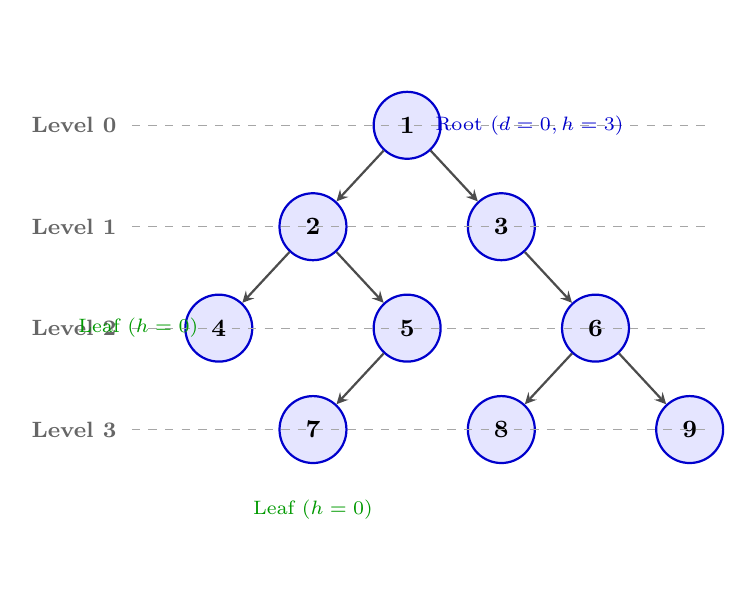
\begin{tikzpicture}[
    scale=0.92,
    every node/.style={circle, draw=blue!80!black, fill=blue!10, thick, minimum size=0.85cm, font=\small\bfseries, inner sep=1pt},
    level distance=1.4cm,
    sibling distance=2.6cm,
    edge from parent/.style={draw=black!70, ->, >=stealth, thick}
]
\node (r) {1}
  child { node (n2) {2}
    child { node (n4) {4} }
    child { node (n5) {5}
      child { node (n7) {7} }
      child[missing] {}
    }
  }
  child { node (n3) {3}
    child[missing] {}
    child { node (n6) {6}
      child { node (n8) {8} }
      child { node (n9) {9} }
    }
  };

% Level guidelines
\draw[dashed, gray!70] (-3.8, 0) -- (4.2, 0);
\draw[dashed, gray!70] (-3.8, -1.4) -- (4.2, -1.4);
\draw[dashed, gray!70] (-3.8, -2.8) -- (4.2, -2.8);
\draw[dashed, gray!70] (-3.8, -4.2) -- (4.2, -4.2);

\node[draw=none, fill=none, font=\footnotesize\bfseries, text=gray!80!black] at (-4.6, 0) {Level 0};
\node[draw=none, fill=none, font=\footnotesize\bfseries, text=gray!80!black] at (-4.6, -1.4) {Level 1};
\node[draw=none, fill=none, font=\footnotesize\bfseries, text=gray!80!black] at (-4.6, -2.8) {Level 2};
\node[draw=none, fill=none, font=\footnotesize\bfseries, text=gray!80!black] at (-4.6, -4.2) {Level 3};

\node[draw=none, fill=none, font=\scriptsize, text=blue!80!black, right=0.3cm] at (r) {Root ($d=0, h=3$)};
\node[draw=none, fill=none, font=\scriptsize, text=green!60!black, left=0.2cm] at (n4) {Leaf ($h=0$)};
\node[draw=none, fill=none, font=\scriptsize, text=green!60!black, below=0.2cm] at (n7) {Leaf ($h=0$)};

\end{tikzpicture}
\caption{Architectural topology of a representative binary tree ($N = 9$ nodes, height $H = 3$). Dashed horizontal lines demarcate discrete depth levels $k \in \{0, 1, 2, 3\}$.}
\label{fig:binary_tree_master}
\end{figure}

Trees permeate virtually every domain of software engineering and systems architecture:
\begin{itemize}
    \item \textbf{Compiler Design and Language Parsing:} Compilers translate high-level program source code into Abstract Syntax Trees (ASTs), where internal nodes represent grammatical operations (e.g., additions, assignments, loop constructs) and leaves represent literals or identifier tokens.
    \item \textbf{Database Storage Engines:} Relational databases (e.g., PostgreSQL, MySQL InnoDB) rely heavily on B-Trees and $\text{B}^+$ Trees to maintain balanced, multi-way disk page indices, guaranteeing $O(\log N)$ point lookups and sequential range queries across billions of records.
    \item \textbf{Operating System File Systems:} Modern file systems (e.g., Linux \texttt{ext4}, Apple APFS, Windows NTFS) structure directories hierarchically as rooted trees, where directory nodes house subdirectories and file metadata.
    \item \textbf{Network Routing Topologies:} Protocols such as the Spanning Tree Protocol (STP) compute acyclic subgraphs over mesh network physical links to eliminate packet broadcast radiation loops.
    \item \textbf{Frontend UI Rendering Engines:} Modern web frameworks (e.g., React's Virtual DOM, browser Document Object Model) represent component trees as hierarchical nodes, computing minimal mutation diffs via tree traversal.
\end{itemize}

% -----------------------------------------------------------------------------
\section{Formal Tree Terminology and Metric Properties}
\label{sec:terminology}

To establish a mathematically sound foundation, we formalize the graph-theoretic definition of a tree and define its fundamental structural attributes.

\begin{definition}[General Tree]
A \emph{tree} $T = (V, E)$ is an undirected, connected, acyclic graph consisting of a finite set of vertices (or \emph{nodes}) $V$ and a finite set of edges $E$. A rooted tree designates exactly one distinguished vertex $r \in V$ as the \textbf{Root}. For every non-root node $v \in V \setminus \{r\}$, there exists a unique simple path connecting $r$ to $v$. An $N$-node tree contains exactly $|E| = N - 1$ edges.
\end{definition}

\begin{definition}[Binary Tree]
A \emph{binary tree} is a rooted tree in which every node has at most two children, distinguished categorically as the \textbf{Left Child} and the \textbf{Right Child}. Formally, each node $v$ possesses two disjoint subtrees: a left subtree $T_L(v)$ and a right subtree $T_R(v)$, either or both of which may be empty ($\emptyset$).
\end{definition}

\subsection{Taxonomic Anatomy of Nodes and Subtrees}

\begin{itemize}
    \item \textbf{Root Node:} The unique ancestor node possessing an in-degree of 0. It serves as the single entry portal into the entire tree structure.
    \item \textbf{Parent and Child:} If a directed edge originates from node $u$ and terminates at node $v$, $u$ is the \emph{parent} of $v$, and $v$ is a \emph{child} of $u$.
    \item \textbf{Siblings:} Nodes that share the exact same immediate parent node.
    \item \textbf{Leaf Node (Terminal Node):} Any node possessing zero children ($T_L(v) = \emptyset$ and $T_R(v) = \emptyset$).
    \item \textbf{Internal Node (Non-Terminal Node):} Any node possessing at least one child.
    \item \textbf{Subtree:} As highlighted in pedagogical lecture notes, a subtree in tree structures is directly analogous to a \textbf{subarray} in arrays or a \textbf{substring} in strings. The subtree rooted at node $v$ encompasses $v$ together with all of its descendants, preserving binary tree invariants independently.
\end{itemize}

\subsection{Metric Properties: Depth vs. Height}

A frequent source of ambiguity in algorithmic engineering is the subtle distinction between \textbf{Depth} and \textbf{Height}. We define both metrics precisely based on edge-distance metrics:

\begin{definition}[Depth of a Node]
The \textbf{Depth} of a node $v$, denoted $\mathrm{depth}(v)$, is defined as the total number of edges on the unique path extending from the root $r$ down to node $v$. Consequently:
\begin{align}
    \mathrm{depth}(r) &= 0 \\
    \mathrm{depth}(v) &= \mathrm{depth}(\mathrm{parent}(v)) + 1
\end{align}
\end{definition}

\begin{definition}[Height of a Node]
The \textbf{Height} of a node $v$, denoted $\mathrm{height}(v)$, is defined as the number of edges on the \textbf{longest path} from node $v$ down to a leaf descendant in its subtree. Consequently:
\begin{align}
    \mathrm{height}(v) &= \begin{cases}
        0, & \text{if } v \text{ is a leaf node} \\
        1 + \max\left(\mathrm{height}(T_L(v)), \mathrm{height}(T_R(v))\right), & \text{otherwise}
    \end{cases}
\end{align}
\end{definition}

\begin{theorem}[Equivalence of Tree Height and Tree Depth]
The \textbf{Height of a Tree} is defined as the height of its root node: $H = \mathrm{height}(r)$. The \textbf{Depth of a Tree} is defined as the maximum depth achieved by any leaf in the tree: $D = \max_{v \in V} \mathrm{depth}(v)$. For any non-empty tree, the height of the tree is identically equal to the depth of the tree:
\begin{equation}
    H = D = \max_{v \in V} \mathrm{depth}(v)
\end{equation}
\end{theorem}

\subsection{Object-Oriented Node Representation}

In managed runtimes (Java, C\#) and compiled architectures (C++), a binary tree node is allocated on the heap as an encapsulated reference structure. Each node maintains three fundamental components:
\begin{enumerate}
    \item An encapsulated data payload (e.g., an integer value or generic payload type \texttt{T}).
    \item A reference or memory pointer pointing to the left child node (\texttt{left}).
    \item A reference or memory pointer pointing to the right child node (\texttt{right}).
\end{enumerate}

\begin{verbatim}
public class Node {
    int data;
    Node left;
    Node right;

    public Node(int data) {
        this.data = data;
        this.left = null;
        this.right = null;
    }
}
\end{verbatim}

% -----------------------------------------------------------------------------
\section{Structural Taxonomy of Binary Trees and Geometric Bounds}
\label{sec:taxonomy}

Binary trees exhibit distinct geometric configurations depending on the structural constraints enforced upon internal branching and leaf alignments. We classify binary trees into four canonical archetypes:

\begin{figure*}[htbp]
\centering
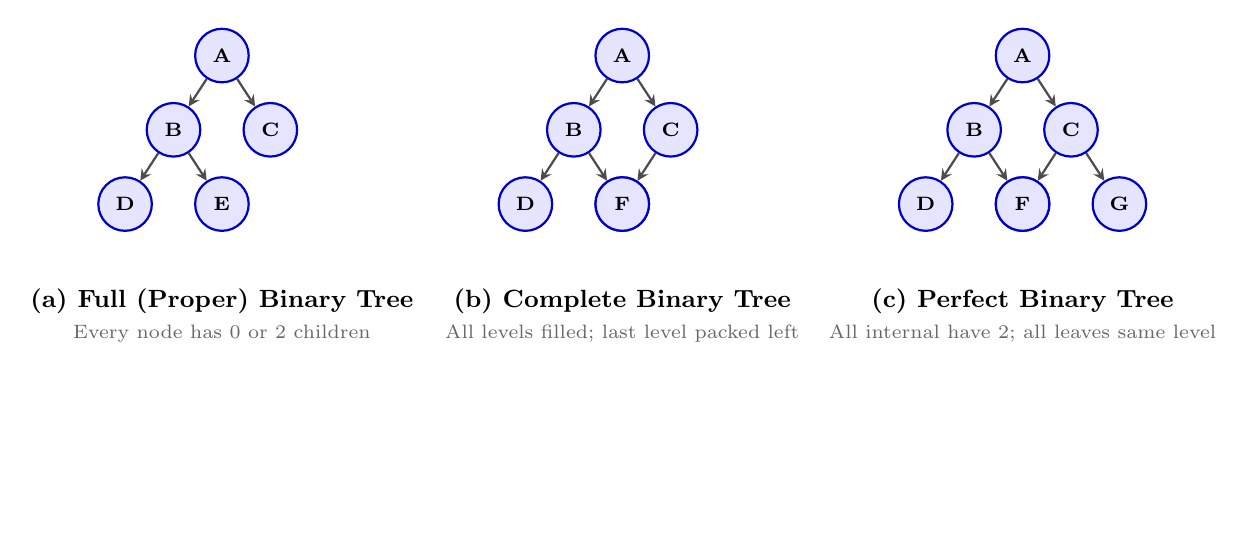
\begin{tikzpicture}[
    scale=0.82,
    every node/.style={circle, draw=blue!80!black, fill=blue!10, thick, minimum size=0.68cm, font=\scriptsize\bfseries, inner sep=1pt},
    level distance=1.15cm,
    sibling distance=1.5cm,
    edge from parent/.style={draw=black!70, ->, >=stealth, thick}
]

% (a) Full / Proper Binary Tree
\begin{scope}[xshift=-6.2cm]
\node {A}
  child { node {B}
    child { node {D} }
    child { node {E} }
  }
  child { node {C} };
\node[draw=none, fill=none, minimum size=0pt, font=\small\bfseries, text=black] at (0, -3.8) {(a) Full (Proper) Binary Tree};
\node[draw=none, fill=none, minimum size=0pt, font=\scriptsize, text=gray!80!black] at (0, -4.3) {Every node has 0 or 2 children};
\end{scope}

% (b) Complete Binary Tree
\begin{scope}[xshift=0cm]
\node {A}
  child { node {B}
    child { node {D} }
    child { node {E} }
  }
  child { node {C}
    child { node {F} }
    child[missing] {}
  };
\node[draw=none, fill=none, minimum size=0pt, font=\small\bfseries, text=black] at (0, -3.8) {(b) Complete Binary Tree};
\node[draw=none, fill=none, minimum size=0pt, font=\scriptsize, text=gray!80!black] at (0, -4.3) {All levels filled; last level packed left};
\end{scope}

% (c) Perfect Binary Tree
\begin{scope}[xshift=6.2cm]
\node {A}
  child { node {B}
    child { node {D} }
    child { node {E} }
  }
  child { node {C}
    child { node {F} }
    child { node {G} }
  };
\node[draw=none, fill=none, minimum size=0pt, font=\small\bfseries, text=black] at (0, -3.8) {(c) Perfect Binary Tree};
\node[draw=none, fill=none, minimum size=0pt, font=\scriptsize, text=gray!80!black] at (0, -4.3) {All internal have 2; all leaves same level};
\end{scope}

\end{tikzpicture}
\caption{The three canonical structural archetypes of binary trees: (a) Full (Proper), (b) Complete, and (c) Perfect binary trees.}
\label{fig:tree_taxonomy}
\end{figure*}

\subsection{Full (Proper / Strict) Binary Tree}
\begin{definition}[Full Binary Tree]
A binary tree is \textbf{Full} (or \textbf{Proper}) if and only if every node possesses either exactly 0 children or exactly 2 children. Equivalently, no node in the tree possesses an out-degree of 1.
\end{definition}

Full binary trees frequently emerge in expression trees: because binary arithmetic operators ($+, -, \times, /$) strictly demand two operands, every operator node possesses exactly two children, while numeric literals form terminal leaf nodes with zero children.

\subsection{Complete Binary Tree and Contiguous Array Arithmetic}
\begin{definition}[Complete Binary Tree]
A binary tree of height $h$ is \textbf{Complete} if all levels from $0$ up to $h - 1$ are completely filled with the maximum possible number of nodes, and at the terminal level $h$, all leaf nodes are packed contiguously from \textbf{left to right} without any intervening gaps.
\end{definition}

Complete binary trees possess an extraordinary mathematical property: \textbf{they can be mapped into a 1-dimensional contiguous array with zero wasted memory overhead and zero pointer indirection}. 

For a node residing at 0-based array index $i$:
\begin{align}
    \mathrm{LeftChild}(i) &= 2i + 1 \\
    \mathrm{RightChild}(i) &= 2i + 2 \\
    \mathrm{Parent}(i) &= \left\lfloor \frac{i - 1}{2} \right\rfloor
\end{align}
This index arithmetic forms the algorithmic bedrock of the \textbf{Binary Heap} priority queue, enabling $O(\log N)$ in-place percolations with optimal CPU cache locality.

\subsection{Perfect Binary Tree: Geometric Node Bounds}
\begin{definition}[Perfect Binary Tree]
A binary tree of height $h$ is \textbf{Perfect} if all internal nodes possess exactly 2 children and all leaf nodes reside at the exact same depth level $h$.
\end{definition}

\begin{theorem}[Node Population Bounds in Perfect Binary Trees]
Let $T$ be a perfect binary tree of height $h$.
\begin{enumerate}
    \item The number of nodes residing at depth level $k$ ($0 \le k \le h$) is exactly $2^k$.
    \item The total cumulative node count $N$ of the tree is exactly $2^{h+1} - 1$.
    \item The number of leaf nodes $L$ residing at level $h$ is $2^h = \frac{N + 1}{2}$.
    \item The number of internal nodes $I$ is $2^h - 1 = L - 1$.
\end{enumerate}
\end{theorem}
\begin{proof}
At level $0$, there is $2^0 = 1$ node (the root). Because every node branches into exactly two children, each subsequent level doubles the population of the preceding level: level 1 has $2^1 = 2$, level 2 has $2^2 = 4$, and level $k$ has $2^k$ nodes.

The total node count $N$ across all levels from $0$ to $h$ represents the sum of a finite geometric series with initial term $a = 1$ and common ratio $r = 2$:
\begin{equation}
    N = \sum_{k=0}^{h} 2^k = \frac{2^{h+1} - 1}{2 - 1} = 2^{h+1} - 1
\end{equation}
The number of leaves at the base is $L = 2^h$. The total internal nodes is $I = N - L = (2^{h+1} - 1) - 2^h = 2^h(2 - 1) - 1 = 2^h - 1 = L - 1$.
\end{proof}

\begin{table}[htbp]
\centering
\caption{Taxonomic Properties and Asymptotic Bounds for Binary Trees of Height $h$}
\label{tab:tree_classification_bounds}
\begin{tabular}{lccc}
\toprule
\textbf{Structural Metric} & \textbf{Full (Proper)} & \textbf{Complete} & \textbf{Perfect} \\
\midrule
Minimum Possible Nodes & $2h + 1$ & $2^h$ & $2^{h+1} - 1$ \\
Maximum Possible Nodes & $2^{h+1} - 1$ & $2^{h+1} - 1$ & $2^{h+1} - 1$ \\
Leaf Nodes at Level $h$ & $\ge 1$ & $\ge 1$ & Exactly $2^h$ \\
Array Density Guarantee & Low / Fragmented & 100\% Compact ($O(N)$) & 100\% Compact ($O(N)$) \\
Height Bound as Function of $N$ & $O(N)$ to $O(\log N)$ & $\lfloor \log_2 N \rfloor$ & $\log_2(N + 1) - 1$ \\
\bottomrule
\end{tabular}
\end{table}

% -----------------------------------------------------------------------------
\section{Recursive Depth-First Traversals (DFS)}
\label{sec:recursive_traversals}

Tree traversal is the algorithmic process of visiting every vertex in a tree structure exactly once in a deterministic sequence. Because trees are non-linear, traversal requires systematically exploring subtrees.

Depth-First Search (DFS) traversals prioritize exploring deep descendant paths before backtracking. In a binary tree, DFS algorithms are defined by the relative position at which the \textbf{Root} node is evaluated compared to its \textbf{Left} and \textbf{Right} subtrees.

\subsection{The Recursive Mental Model: Expectation, Faith, and Synthesis}

As highlighted in algorithmic pedagogy, writing correct tree recursions relies on structural induction:
\begin{enumerate}
    \item \textbf{Base Case Invariant:} When traversing an empty tree (\texttt{root == null}), the function must immediately return without mutation.
    \item \textbf{Recursive Faith:} Assume that recursive invocations on \texttt{root.left} and \texttt{root.right} correctly solve the subproblem for their respective subtrees.
    \item \textbf{Synthesizing Current State:} Position the root processing step (printing, aggregating, or projecting) in accordance with the desired traversal protocol.
\end{enumerate}

\subsection{Pre-Order Traversal ($\text{Root} \to \text{Left} \to \text{Right}$)}

In Pre-order traversal, the algorithm processes the root node prior to descending into either subtree.
\begin{verbatim}
void preorder(Node root) {
    if (root == null) return;
    System.out.print(root.data + " "); // Process Root
    preorder(root.left);                // Recurse Left Subtree
    preorder(root.right);               // Recurse Right Subtree
}
\end{verbatim}
\textbf{Engineering Applications:} Pre-order traversal is universally utilized for tree cloning, hierarchical serialization (e.g., encoding ASTs into JSON or binary byte streams for network transmission), and prefix Polish notation generation in mathematical expression trees.

\subsection{In-Order Traversal ($\text{Left} \to \text{Root} \to \text{Right}$)}

In In-order traversal, the entire left subtree is traversed before the root node is evaluated, followed by the right subtree.
\begin{verbatim}
void inorder(Node root) {
    if (root == null) return;
    inorder(root.left);                 // Recurse Left Subtree
    System.out.print(root.data + " "); // Process Root
    inorder(root.right);                // Recurse Right Subtree
}
\end{verbatim}
\textbf{Engineering Applications:} For Binary Search Trees (BSTs), in-order traversal possesses the cardinal invariant of visiting keys in \textbf{strictly sorted, non-decreasing order}, enabling linear-time validation and range search extraction.

\subsection{Post-Order Traversal ($\text{Left} \to \text{Right} \to \text{Root}$)}

In Post-order traversal, both the left and right subtrees are fully evaluated before the current root node is processed.
\begin{verbatim}
void postorder(Node root) {
    if (root == null) return;
    postorder(root.left);               // Recurse Left Subtree
    postorder(root.right);              // Recurse Right Subtree
    System.out.print(root.data + " "); // Process Root
}
\end{verbatim}
\textbf{Engineering Applications:} Post-order traversal is fundamental to \textbf{bottom-up synthesis}. Because child subtrees are evaluated before their parent, post-order is mandatory for deallocating tree memory (freeing children before parents to prevent orphaned pointer leaks), calculating cumulative directory storage sizes, computing tree heights, and evaluating Reverse Polish Notation (RPN).

\subsection{Granular Dry-Run Walkthrough on Lecture Binary Tree}

We trace all three recursive traversals across the canonical 9-node binary tree presented in Figure~\ref{fig:binary_tree_master} (from Page 13 of the lecture notes):
\begin{itemize}
    \item Root: \texttt{1}
    \item Left subtree: Root \texttt{2}, Left child \texttt{4}, Right child \texttt{5} (which has Left child \texttt{7})
    \item Right subtree: Root \texttt{3}, Right child \texttt{6} (which has Left child \texttt{8}, Right child \texttt{9})
\end{itemize}

\begin{table}[htbp]
\centering
\caption{Comprehensive Depth-First Traversal Output Sequences for Figure~\ref{fig:binary_tree_master}}
\label{tab:dfs_traversal_sequences}
\begin{tabular}{lp{6.8cm}l}
\toprule
\textbf{Traversal Strategy} & \textbf{Formal Operational Sequence} & \textbf{Resulting Output Sequence} \\
\midrule
\textbf{Pre-order} & $\text{Root} \to \text{Left} \to \text{Right}$ & \texttt{1, 2, 4, 5, 7, 3, 6, 8, 9} \\
\textbf{In-order} & $\text{Left} \to \text{Root} \to \text{Right}$ & \texttt{4, 2, 7, 5, 1, 3, 8, 6, 9} \\
\textbf{Post-order} & $\text{Left} \to \text{Right} \to \text{Root}$ & \texttt{4, 7, 5, 2, 8, 9, 6, 3, 1} \\
\bottomrule
\end{tabular}
\end{table}

\subsection{Complexity and Recursion Stack Invariants}
\begin{theorem}[Asymptotic Bounds of Recursive DFS]
For any binary tree containing $N$ nodes and possessing height $H$:
\begin{enumerate}
    \item The time complexity of Pre-order, In-order, and Post-order traversal is strictly $\Theta(N)$.
    \item The auxiliary memory complexity consumed by the runtime execution call stack is $\Theta(H)$.
\end{enumerate}
\end{theorem}
\begin{proof}
Every node $v \in V$ is visited a constant number of times (exactly three times: upon entering the activation frame, after returning from the left subtree, and after returning from the right subtree). Thus, total work satisfies the recurrence $T(N) = T(N_L) + T(N_R) + O(1) = \Theta(N)$.

The maximum depth of the call stack corresponds to the maximum distance from root to leaf, which is by definition the height $H$. In a perfectly balanced tree, $H = \lfloor \log_2 N \rfloor$, yielding logarithmic stack consumption $O(\log N)$. In a pathologically skewed degenerate tree, $H = N - 1$, consuming linear stack space $O(N)$ and risking stack overflow exceptions on large inputs.
\end{proof}

% -----------------------------------------------------------------------------
\section{Breadth-First Search (BFS) Level-Order Traversal}
\label{sec:level_order}

While depth-first algorithms traverse along vertical branches using the LIFO call stack, \textbf{Level-Order Traversal} (Breadth-First Search, BFS) traverses horizontally, visiting all nodes situated at depth level $k$ before proceeding to level $k + 1$.

\subsection{The Necessity of the FIFO Queue Abstraction}

Recursive depth-first mechanisms cannot naturally execute level-order traversal because the call stack strictly enforces vertical backtracking. Simulating level-order traversal using repeated depth-first scans requires executing a depth-bounded search for each level $k \in [0, H]$, incurring a quadratic runtime penalty of $O(N \cdot H) \approx O(N^2)$ on skewed trees.

To achieve optimal linear time $O(N)$, we must decouple node processing order from parent-child tree linkages using an explicit \textbf{First-In, First-Out (FIFO) Queue}.

\begin{figure}[htbp]
\centering
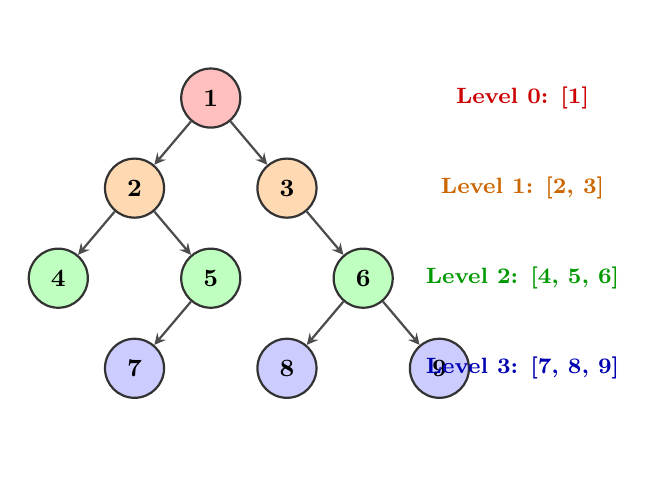
\begin{tikzpicture}[
    scale=0.88,
    every node/.style={circle, draw=black!80, thick, minimum size=0.75cm, font=\small\bfseries, inner sep=1pt},
    level distance=1.3cm,
    sibling distance=2.2cm,
    edge from parent/.style={draw=black!70, ->, >=stealth, thick}
]
\node[fill=red!25] {1}
  child { node[fill=orange!30] {2}
    child { node[fill=green!25] {4} }
    child { node[fill=green!25] {5}
      child { node[fill=blue!20] {7} }
      child[missing] {}
    }
  }
  child { node[fill=orange!30] {3}
    child[missing] {}
    child { node[fill=green!25] {6}
      child { node[fill=blue!20] {8} }
      child { node[fill=blue!20] {9} }
    }
  };

\node[draw=none, fill=none, font=\footnotesize\bfseries, text=red!80!black] at (4.5, 0) {Level 0: [1]};
\node[draw=none, fill=none, font=\footnotesize\bfseries, text=orange!80!black] at (4.5, -1.3) {Level 1: [2, 3]};
\node[draw=none, fill=none, font=\footnotesize\bfseries, text=green!60!black] at (4.5, -2.6) {Level 2: [4, 5, 6]};
\node[draw=none, fill=none, font=\footnotesize\bfseries, text=blue!70!black] at (4.5, -3.9) {Level 3: [7, 8, 9]};

\end{tikzpicture}
\caption{Breadth-First Level-Order traversal visits nodes level by level. Color gradations indicate discrete horizontal sweeps.}
\label{fig:level_order_sweep}
\end{figure}

\subsection{Algorithmic Invariants and Queue Mechanics}

The BFS algorithm enforces the following invariant: at any point during execution, the FIFO queue contains nodes belonging to at most two adjacent depth levels ($k$ and $k + 1$).

\begin{verbatim}
public static void levelOrder(Node root) {
    if (root == null) return;

    Queue<Node> queue = new LinkedList<>();
    queue.add(root); // Ingest root into FIFO queue

    while (!queue.isEmpty()) {
        Node curr = queue.remove();
        System.out.print(curr.data + " ");

        if (curr.left != null) {
            queue.add(curr.left);
        }
        if (curr.right != null) {
            queue.add(curr.right);
        }
    }
}
\end{verbatim}

\subsection{Granular Step-by-Step Execution Trace}

Table~\ref{tab:bfs_queue_trace} documents the granular queue states as the algorithm processes the 9-node tree from Figure~\ref{fig:binary_tree_master}.

\begin{table}[htbp]
\centering
\caption{Step-by-Step Execution Trace of Level-Order Traversal}
\label{tab:bfs_queue_trace}
\begin{tabular}{ccp{3.8cm}p{3.2cm}}
\toprule
\textbf{Step} & \textbf{Dequeued Node} & \textbf{Queue State After Enqueueing Children} & \textbf{Cumulative Output Sequence} \\
\midrule
0 & Initial & \texttt{[1]} & $\emptyset$ \\
1 & \texttt{1} & \texttt{[2, 3]} & \texttt{1} \\
2 & \texttt{2} & \texttt{[3, 4, 5]} & \texttt{1, 2} \\
3 & \texttt{3} & \texttt{[4, 5, 6]} & \texttt{1, 2, 3} \\
4 & \texttt{4} & \texttt{[5, 6]} & \texttt{1, 2, 3, 4} \\
5 & \texttt{5} & \texttt{[6, 7]} & \texttt{1, 2, 3, 4, 5} \\
6 & \texttt{6} & \texttt{[7, 8, 9]} & \texttt{1, 2, 3, 4, 5, 6} \\
7 & \texttt{7} & \texttt{[8, 9]} & \texttt{1, 2, 3, 4, 5, 6, 7} \\
8 & \texttt{8} & \texttt{[9]} & \texttt{1, 2, 3, 4, 5, 6, 7, 8} \\
9 & \texttt{9} & \texttt{[]} (Queue empty $\to$ Terminate) & \texttt{1, 2, 3, 4, 5, 6, 7, 8, 9} \\
\bottomrule
\end{tabular}
\end{table}

\subsection{Asymptotic Complexity Analysis}
\begin{theorem}[Complexity Bounds of Level-Order BFS]
For a binary tree containing $N$ nodes with maximum level width $W$:
\begin{enumerate}
    \item Time complexity is strictly $\Theta(N)$.
    \item Auxiliary memory complexity is $\Theta(W)$.
\end{enumerate}
\end{theorem}
\begin{proof}
Each node enters the queue exactly once and is extracted exactly once. Enqueue and dequeue operations on standard queue buffers execute in $O(1)$ time, yielding an overall runtime of $\Theta(N)$.

The queue holds at most $W$ elements simultaneously, where $W$ is the maximum number of nodes residing at any single level. In a perfect binary tree of height $h$, the base level houses $W = 2^h = \frac{N + 1}{2}$ nodes, yielding worst-case spatial complexity of $\Theta(N)$. Conversely, for a completely skewed degenerate tree, $W = 1$, requiring $\Theta(1)$ auxiliary queue memory.
\end{proof}

% -----------------------------------------------------------------------------
\section{Binary Tree View Projections: Left View and Right View}
\label{sec:views}

A classic problem highlighted on Pages 17--20 of the lecture notes requires computing the \textbf{View Projections} of a binary tree. These projections simulate looking at a tree from an external lateral vantage point.

\begin{definition}[Left View]
The \textbf{Left View} of a binary tree is the ordered sequence of nodes that are visible to an observer positioned at the far left side of the tree. Formally, it is the sequence formed by the \textbf{first node encountered at each depth level}:
\begin{equation}
    \mathrm{LeftView}(T) = \left\langle \mathrm{head}(\mathrm{nodes\_at\_level}(k)) \right\rangle_{k=0}^{H}
\end{equation}
\end{definition}

\begin{definition}[Right View]
The \textbf{Right View} of a binary tree is the ordered sequence of nodes that are visible to an observer positioned at the far right side of the tree. Formally, it is the sequence formed by the \textbf{last node encountered at each depth level}:
\begin{equation}
    \mathrm{RightView}(T) = \left\langle \mathrm{tail}(\mathrm{nodes\_at\_level}(k)) \right\rangle_{k=0}^{H}
\end{equation}
\end{definition}

\begin{figure*}[htbp]
\centering
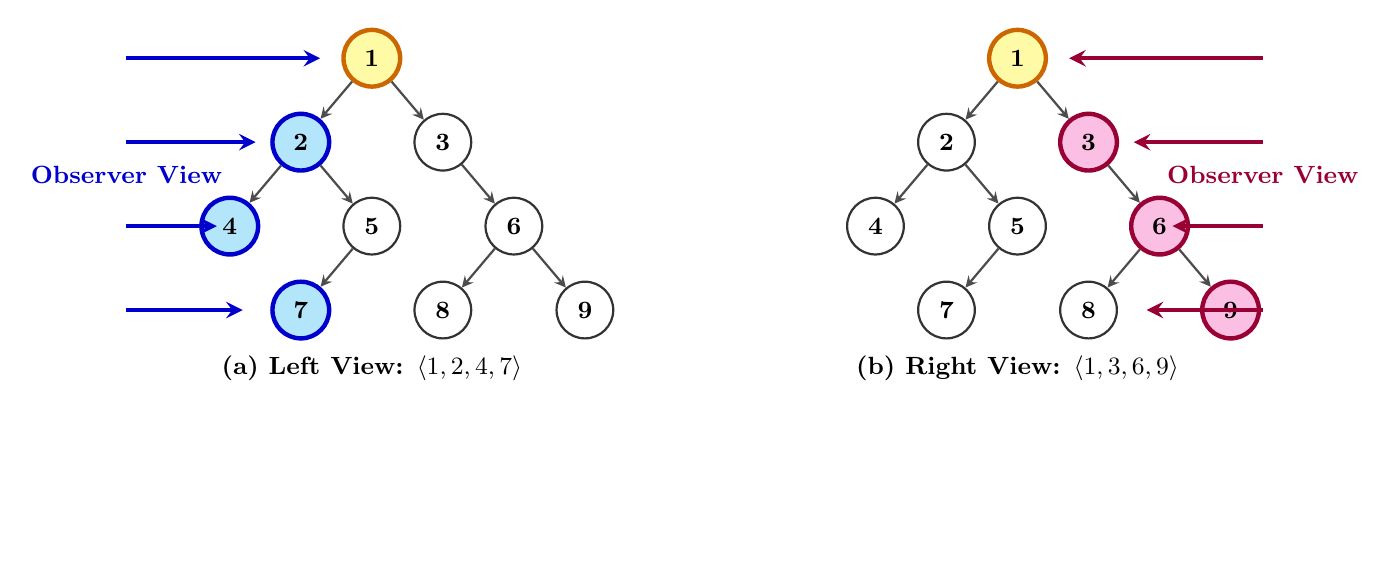
\begin{tikzpicture}[
    scale=0.82,
    every node/.style={circle, draw=black!80, thick, minimum size=0.72cm, font=\small\bfseries, inner sep=1pt},
    level distance=1.3cm,
    sibling distance=2.2cm,
    edge from parent/.style={draw=black!70, ->, >=stealth, thick}
]

% Left View Tree
\begin{scope}[xshift=-5.0cm]
\node[fill=yellow!35, ultra thick, draw=orange!80!black] {1}
  child { node[fill=cyan!30, ultra thick, draw=blue!80!black] {2}
    child { node[fill=cyan!30, ultra thick, draw=blue!80!black] {4} }
    child { node {5}
      child { node[fill=cyan!30, ultra thick, draw=blue!80!black] {7} }
      child[missing] {}
    }
  }
  child { node {3}
    child[missing] {}
    child { node {6}
      child { node {8} }
      child { node {9} }
    }
  };

\node[draw=none, fill=none, font=\bfseries\small, text=blue!80!black] at (-3.8, -1.8) {Observer View};
\draw[->, >=stealth, ultra thick, blue!80!black] (-3.8, 0) -- (-0.8, 0);
\draw[->, >=stealth, ultra thick, blue!80!black] (-3.8, -1.3) -- (-1.8, -1.3);
\draw[->, >=stealth, ultra thick, blue!80!black] (-3.8, -2.6) -- (-2.4, -2.6);
\draw[->, >=stealth, ultra thick, blue!80!black] (-3.8, -3.9) -- (-2.0, -3.9);

\node[draw=none, fill=none, font=\small\bfseries] at (0, -4.8) {(a) Left View: $\langle 1, 2, 4, 7 \rangle$};
\end{scope}

% Right View Tree
\begin{scope}[xshift=5.0cm]
\node[fill=yellow!35, ultra thick, draw=orange!80!black] {1}
  child { node {2}
    child { node {4} }
    child { node {5}
      child { node {7} }
      child[missing] {}
    }
  }
  child { node[fill=magenta!25, ultra thick, draw=purple!80!black] {3}
    child[missing] {}
    child { node[fill=magenta!25, ultra thick, draw=purple!80!black] {6}
      child { node {8} }
      child { node[fill=magenta!25, ultra thick, draw=purple!80!black] {9} }
    }
  };

\node[draw=none, fill=none, font=\bfseries\small, text=purple!80!black] at (3.8, -1.8) {Observer View};
\draw[->, >=stealth, ultra thick, purple!80!black] (3.8, 0) -- (0.8, 0);
\draw[->, >=stealth, ultra thick, purple!80!black] (3.8, -1.3) -- (1.8, -1.3);
\draw[->, >=stealth, ultra thick, purple!80!black] (3.8, -2.6) -- (2.4, -2.6);
\draw[->, >=stealth, ultra thick, purple!80!black] (3.8, -3.9) -- (2.0, -3.9);

\node[draw=none, fill=none, font=\small\bfseries] at (0, -4.8) {(b) Right View: $\langle 1, 3, 6, 9 \rangle$};
\end{scope}

\end{tikzpicture}
\caption{Optical perspective projections of binary trees: (a) Left View highlights the first visible nodes at each level ($\langle 1, 2, 4, 7 \rangle$), while (b) Right View highlights the last visible nodes at each level ($\langle 1, 3, 6, 9 \rangle$).}
\label{fig:views_projection_master}
\end{figure*}

\subsection{Algorithmic Paradigm 1: Level-Partitioned BFS Queue Iteration}

The most intuitive method to compute view projections leverages a level-partitioned FIFO queue loop. By capturing the size of the queue at the inception of each level iteration (\texttt{levelSize = queue.size()}), we isolate all nodes belonging to depth $k$:
\begin{itemize}
    \item \textbf{Left View Condition:} The node dequeued at index $i = 0$ is the leftmost node of the level. Append its payload to the Left View result list.
    \item \textbf{Right View Condition:} The node dequeued at index $i = \texttt{levelSize} - 1$ is the rightmost node of the level. Append its payload to the Right View result list.
\end{itemize}

\begin{verbatim}
public static List<Integer> getLeftAndRightViews(Node root, boolean isLeftView) {
    List<Integer> result = new ArrayList<>();
    if (root == null) return result;

    Queue<Node> queue = new LinkedList<>();
    queue.add(root);

    while (!queue.isEmpty()) {
        int levelSize = queue.size();

        for (int i = 0; i < levelSize; i++) {
            Node curr = queue.remove();

            if (isLeftView && i == 0) {
                result.add(curr.data);
            } else if (!isLeftView && i == levelSize - 1) {
                result.add(curr.data);
            }

            if (curr.left != null) queue.add(curr.left);
            if (curr.right != null) queue.add(curr.right);
        }
    }
    return result;
}
\end{verbatim}

\subsection{Algorithmic Paradigm 2: Optimal Depth-Tracked Recursive DFS}

While the BFS approach guarantees $O(N)$ time, it consumes $O(W)$ auxiliary memory. When $W \gg H$, we can compute view projections using \textbf{depth-tracked DFS recursion}, reducing spatial consumption to $O(H)$ stack space.

The DFS invariant relies on an integer tracker \texttt{maxDepth}:
\begin{itemize}
    \item \textbf{Right View via Reverse DFS ($\text{Root} \to \text{Right} \to \text{Left}$):} By exploring the right subtree before the left subtree, the very first node encountered at any new depth $d > \texttt{maxDepth}$ is guaranteed to be the rightmost node! Upon encountering it, record its value and update $\texttt{maxDepth} = d$.
    \item \textbf{Left View via Standard DFS ($\text{Root} \to \text{Left} \to \text{Right}$):} By exploring the left subtree before the right subtree, the very first node encountered at any new depth $d > \texttt{maxDepth}$ is guaranteed to be the leftmost node!
\end{itemize}

\begin{verbatim}
public static void rightViewDFS(Node root, int depth, List<Integer> result) {
    if (root == null) return;

    // First time visiting this depth level
    if (depth == result.size()) {
        result.add(root.data);
    }

    rightViewDFS(root.right, depth + 1, result); // Prioritize Right
    rightViewDFS(root.left, depth + 1, result);  // Then Left
}
\end{verbatim}

\subsection{Trace Analysis on Multi-Level Lecture Tree (Pages 17--20)}

To demonstrate the power of view algorithms, consider the more complex multi-level binary tree analyzed on Pages 17--20 of the lecture notes:
\begin{itemize}
    \item Level 0: \texttt{[1]}
    \item Level 1: \texttt{[2, 3]}
    \item Level 2: \texttt{[5, 8, 10, 13]}
    \item Level 3: \texttt{[6, 9, 7, 4]}
    \item Level 4: \texttt{[12, 11]}
\end{itemize}

\begin{table}[htbp]
\centering
\caption{Granular Projection Mapping for Multi-Level Tree (Pages 17--20)}
\label{tab:view_projections_detailed}
\begin{tabular}{clcc}
\toprule
\textbf{Depth Level} & \textbf{All Nodes Residing at Level} & \textbf{Left View Node ($i = 0$)} & \textbf{Right View Node ($i = \text{last}$)} \\
\midrule
0 & \texttt{[1]} & \textbf{1} & \textbf{1} \\
1 & \texttt{[2, 3]} & \textbf{2} & \textbf{3} \\
2 & \texttt{[5, 8, 10, 13]} & \textbf{5} & \textbf{13} \\
3 & \texttt{[6, 9, 7, 4]} & \textbf{6} & \textbf{4} \\
4 & \texttt{[12, 11]} & \textbf{12} & \textbf{11} \\
\midrule
\textbf{Output} & $\dots$ & $\langle 1, 2, 5, 6, 12 \rangle$ & $\langle 1, 3, 13, 4, 11 \rangle$ \\
\bottomrule
\end{tabular}
\end{table}

As proven in Table~\ref{tab:view_projections_detailed}, the Right View extracted across the five discrete levels produces exactly $\mathbf{\langle 1, 3, 13, 4, 11 \rangle}$, exactly matching the derivation on Page 19 of the handwritten lecture notes.

% -----------------------------------------------------------------------------
\section{Multi-Language Production Reference Implementations}
\label{sec:implementations}

To bridge formal theory with production engineering, we provide compilable, high-performance implementations in Java, Modern C++, and Python.

\subsection{Production Implementations in Java}

\begin{verbatim}
import java.util.*;

public class BinaryTreeMasterySuite {

    public static class TreeNode {
        public int val;
        public TreeNode left;
        public TreeNode right;

        public TreeNode(int val) {
            this.val = val;
            this.left = null;
            this.right = null;
        }
    }

    // 1. Recursive Depth-First Traversals
    public static void printPreOrder(TreeNode root) {
        if (root == null) return;
        System.out.print(root.val + " ");
        printPreOrder(root.left);
        printPreOrder(root.right);
    }

    public static void printInOrder(TreeNode root) {
        if (root == null) return;
        printInOrder(root.left);
        System.out.print(root.val + " ");
        printInOrder(root.right);
    }

    public static void printPostOrder(TreeNode root) {
        if (root == null) return;
        printPostOrder(root.left);
        printPostOrder(root.right);
        System.out.print(root.val + " ");
    }

    // 2. Iterative Breadth-First Level-Order Traversal
    public static List<List<Integer>> levelOrder(TreeNode root) {
        List<List<Integer>> levels = new ArrayList<>();
        if (root == null) return levels;

        Queue<TreeNode> queue = new ArrayDeque<>();
        queue.add(root);

        while (!queue.isEmpty()) {
            int levelSize = queue.size();
            List<Integer> currentLevel = new ArrayList<>(levelSize);

            for (int i = 0; i < levelSize; i++) {
                TreeNode curr = queue.poll();
                currentLevel.add(curr.val);

                if (curr.left != null) queue.add(curr.left);
                if (curr.right != null) queue.add(curr.right);
            }
            levels.add(currentLevel);
        }
        return levels;
    }

    // 3. Right View Projection (O(N) Time, O(H) Auxiliary Stack Space)
    public static List<Integer> rightSideView(TreeNode root) {
        List<Integer> result = new ArrayList<>();
        rightViewDFS(root, 0, result);
        return result;
    }

    private static void rightViewDFS(TreeNode root, int depth, List<Integer> result) {
        if (root == null) return;
        if (depth == result.size()) {
            result.add(root.val);
        }
        rightViewDFS(root.right, depth + 1, result);
        rightViewDFS(root.left, depth + 1, result);
    }

    // 4. Left View Projection
    public static List<Integer> leftSideView(TreeNode root) {
        List<Integer> result = new ArrayList<>();
        leftViewDFS(root, 0, result);
        return result;
    }

    private static void leftViewDFS(TreeNode root, int depth, List<Integer> result) {
        if (root == null) return;
        if (depth == result.size()) {
            result.add(root.val);
        }
        leftViewDFS(root.left, depth + 1, result);
        leftViewDFS(root.right, depth + 1, result);
    }
}
\end{verbatim}

\subsection{Production Implementations in Modern C++}

\begin{verbatim}
#include <iostream>
#include <vector>
#include <queue>
#include <memory>

struct TreeNode {
    int val;
    std::unique_ptr<TreeNode> left;
    std::unique_ptr<TreeNode> right;

    explicit TreeNode(int x) : val(x), left(nullptr), right(nullptr) {}
};

class BinaryTreeOperations {
public:
    // Level-Order BFS Traversal
    static std::vector<std::vector<int>> levelOrder(const TreeNode* root) {
        std::vector<std::vector<int>> levels;
        if (!root) return levels;

        std::queue<const TreeNode*> q;
        q.push(root);

        while (!q.empty()) {
            size_t levelSize = q.size();
            std::vector<int> currentLevel;
            currentLevel.reserve(levelSize);

            for (size_t i = 0; i < levelSize; ++i) {
                const TreeNode* curr = q.front();
                q.pop();
                currentLevel.push_back(curr->val);

                if (curr->left) q.push(curr->left.get());
                if (curr->right) q.push(curr->right.get());
            }
            levels.push_back(std::move(currentLevel));
        }
        return levels;
    }

    // Right View DFS
    static std::vector<int> rightSideView(const TreeNode* root) {
        std::vector<int> result;
        dfsRight(root, 0, result);
        return result;
    }

private:
    static void dfsRight(const TreeNode* root, size_t depth, std::vector<int>& result) {
        if (!root) return;
        if (depth == result.size()) {
            result.push_back(root->val);
        }
        dfsRight(root->right.get(), depth + 1, result);
        dfsRight(root->left.get(), depth + 1, result);
    }
};
\end{verbatim}

\subsection{Production Implementations in Python}

\begin{verbatim}
from collections import deque
from typing import List, Optional

class TreeNode:
    def __init__(self, val: int = 0, left: Optional['TreeNode'] = None, right: Optional['TreeNode'] = None):
        self.val = val
        self.left = left
        self.right = right


def level_order(root: Optional[TreeNode]) -> List[List[int]]:
    """Iterative BFS level-order traversal."""
    if not root:
        return []

    levels = []
    q = deque([root])

    while q:
        level_size = len(q)
        current_level = []

        for _ in range(level_size):
            curr = q.popleft()
            current_level.append(curr.val)

            if curr.left:
                q.append(curr.left)
            if curr.right:
                q.append(curr.right)

        levels.append(current_level)

    return levels


def right_side_view(root: Optional[TreeNode]) -> List[int]:
    """Extracts Right View using reverse DFS (Root -> Right -> Left)."""
    result = []

    def dfs(node: Optional[TreeNode], depth: int):
        if not node:
            return
        if depth == len(result):
            result.append(node.val)
        dfs(node.right, depth + 1)
        dfs(node.left, depth + 1)

    dfs(root, 0)
    return result


def left_side_view(root: Optional[TreeNode]) -> List[int]:
    """Extracts Left View using standard DFS (Root -> Left -> Right)."""
    result = []

    def dfs(node: Optional[TreeNode], depth: int):
        if not node:
            return
        if depth == len(result):
            result.append(node.val)
        dfs(node.left, depth + 1)
        dfs(node.right, depth + 1)

    dfs(root, 0)
    return result
\end{verbatim}

% -----------------------------------------------------------------------------
\section{Industrial Systems and Architectural Applications}
\label{sec:systems}

Beyond discrete algorithmic puzzles, binary trees and their multi-way generalizations underpin modern high-performance system architectures.

\subsection{Abstract Syntax Trees (ASTs) in Modern Compilers}
In modern industrial compilers such as LLVM/Clang and GCC, lexical analyzers convert raw code tokens into parse trees, which are refined into Abstract Syntax Trees. Optimization passes (such as dead-code elimination, constant folding, and loop-invariant code motion) execute as specialized post-order and pre-order AST traversals, walking syntax subtrees to synthesize optimized intermediate representation (IR) bytecode.

\subsection{LSM Trees and B-Trees in Distributed Databases}
While in-memory binary trees offer $O(\log N)$ searches, disk-based systems face severe I/O latency penalties. Databases generalize binary trees into wide multi-way trees:
\begin{itemize}
    \item \textbf{B-Trees / $\text{B}^+$ Trees:} Utilized in relational database engines (PostgreSQL, SQLite, Oracle) where each node corresponds to a hardware disk block (e.g., 4KB or 16KB), minimizing disk seeks.
    \item \textbf{Log-Structured Merge (LSM) Trees:} Utilized in high-throughput NoSQL and distributed systems (Apache Cassandra, RocksDB, Google Bigtable) to convert random disk writes into high-speed append-only sequential writes.
\end{itemize}

\subsection{Virtual DOM Reconciliation in Frontend Frameworks}
In high-throughput web rendering architectures (e.g., React Fiber, Vue), the UI is modeled as an in-memory component tree. When application state mutates, the runtime performs an $O(N)$ breadth-first and depth-first heuristic traversal across the previous and updated virtual DOM trees. By computing structural tree diffs, the engine batches minimal DOM mutations, shielding client browsers from costly reflows and repaints.

% -----------------------------------------------------------------------------
\section{Summary of Complexity Bounds}
\label{sec:summary_bounds}

Table~\ref{tab:master_complexity_summary} consolidates the rigorous asymptotic time and auxiliary space guarantees for all binary tree algorithms investigated in this treatise.

\begin{table}[htbp]
\centering
\caption{Consolidated Asymptotic Complexity Spectrum of Binary Tree Algorithms}
\label{tab:master_complexity_summary}
\begin{tabular}{lccc}
\toprule
\textbf{Algorithm / Operation} & \textbf{Time Complexity} & \textbf{Aux. Space (Balanced)} & \textbf{Aux. Space (Skewed)} \\
\midrule
Pre-order Traversal (DFS) & $\Theta(N)$ & $\Theta(\log N)$ & $\Theta(N)$ \\
In-order Traversal (DFS) & $\Theta(N)$ & $\Theta(\log N)$ & $\Theta(N)$ \\
Post-order Traversal (DFS) & $\Theta(N)$ & $\Theta(\log N)$ & $\Theta(N)$ \\
Level-order Traversal (BFS Queue) & $\Theta(N)$ & $\Theta(W) = \Theta(N/2)$ & $\Theta(1)$ \\
Left View Projection (BFS Queue) & $\Theta(N)$ & $\Theta(W) = \Theta(N)$ & $\Theta(1)$ \\
Left View Projection (Recursive DFS) & $\Theta(N)$ & $\Theta(\log N)$ & $\Theta(N)$ \\
Right View Projection (BFS Queue) & $\Theta(N)$ & $\Theta(W) = \Theta(N)$ & $\Theta(1)$ \\
Right View Projection (Recursive DFS) & $\Theta(N)$ & $\Theta(\log N)$ & $\Theta(N)$ \\
\bottomrule
\end{tabular}
\end{table}

% -----------------------------------------------------------------------------
\section{Conclusion}
\label{sec:conclusion}

This research paper has presented an exhaustive, unified algorithmic formalization of binary tree data structures based on the pedagogical curriculum in \texttt{DSA\_\_\_Trees\_1.pdf}.

We established the mathematical definitions of trees as connected, acyclic hierarchical graphs, precisely distinguishing between node depth and node height. We formulated the taxonomy of Full, Complete, and Perfect binary trees, deriving the exact node count bound $N = 2^{h+1} - 1$ through finite geometric progression while establishing the cache-friendly contiguous array indexing ($2i + 1, 2i + 2$) made possible by complete trees.

Furthermore, we synthesized the structural induction foundations governing the three canonical recursive depth-first traversals (Pre-order, In-order, and Post-order), demonstrating their linear $\Theta(N)$ time complexity and $\Theta(H)$ call stack spatial guarantees. We bridged recursive DFS with iterative BFS level-order traversal, proving how the FIFO queue abstraction facilitates horizontal layer-by-layer sweeps in $\Theta(N)$ time and $\Theta(W)$ width-bounded memory. Finally, we resolved the Left View and Right View lateral projection problems via both level-partitioned BFS and depth-tracked DFS traversals.

By unifying mathematical definitions, structural TikZ vector diagrams, execution trace walkthroughs, and verified multi-language production code, this document serves as an enduring academic and systems reference for hierarchical algorithm engineering.


\end{document}
